%%%%%%%%%%%%%%%%%%%%%%%%%%%%%%%%%%%%%%%%%%%%%%%%%%%%%%%%%%%%%%%%%%%%%%%%
%                                                                      %
%     File: Thesis_FrontCover.tex                                      %
%     Tex Master: Thesis.tex                                           %
%                                                                      %
%     Author: Andre C. Marta                                           %
%     Last modified : 27 Feb 2024                                      %
%                                                                      %
%%%%%%%%%%%%%%%%%%%%%%%%%%%%%%%%%%%%%%%%%%%%%%%%%%%%%%%%%%%%%%%%%%%%%%%%

\thispagestyle {empty}

% IST Logo - Signature A
% parameters: bb=llx lly urx ury (bounding box), width=h_length, height=v_length, angle=angle, scale=factor, clip=true/false, draft=true/false. 

\includegraphics[bb=9.5cm 11cm 0cm 0cm,scale=0.29]{Figures/ist_logo.png}

\begin{center}
%
% Figure (Image or plot)
\vspace{2.5cm}
% height = 50 mm
% the tethered system as displayed in Foxglove (as in Figure 4.6a)
\reflectbox{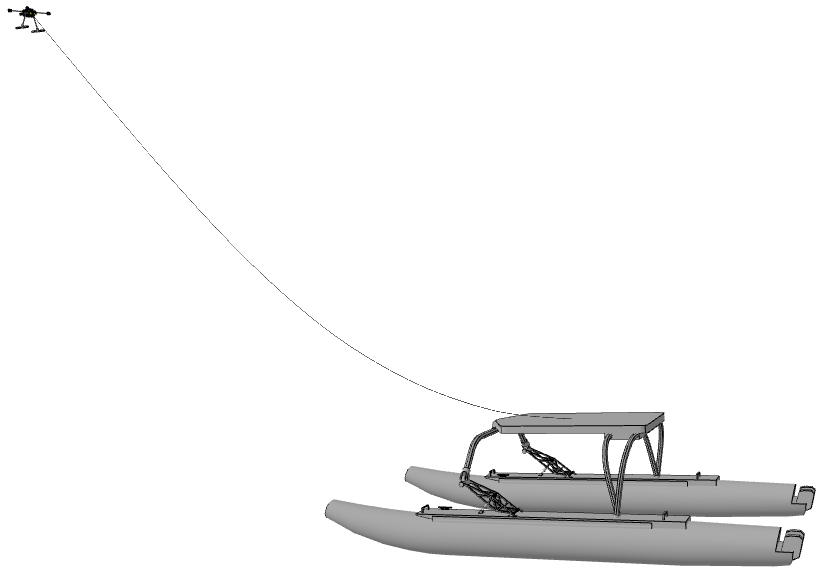
\includegraphics[height=50mm]{Implementation/figures/01_simulation_environment/drone_foxglove_side.png}}

% Title, author and degree
\vspace{1.0cm}
{\FontLb Cooperative control of a tethered drone and surface vessel for sustained presence at sea} \\ % <<<<< EDIT TITLE
%\vspace{0.2cm}
%{\FontMn Subtitle (optional)} \\
\vspace{1.9cm}
% \vspace{2.6cm}
{\FontMb Tomás Grossinho Esteves} \\ % <<<<< EDIT NAME
\vspace{2.0cm}
{\FontSn \coverThesis} \\
% {\FontSn 2nd Cycle Integrated Project} \\
\vspace{0.3cm}
{\FontLb Electrical and Computer Engineering} \\ % <<<<< EDIT COURSE
\vspace{1.0cm}
{\FontSn %
\begin{tabular}{ll}
 \coverSupervisors: & Doctor David Alexandre Cabecinhas \\ % <<<<< EDIT NAME
                    & Doctor Rita Maria Mendes de Almeida Correia da Cunha    % <<<<< EDIT NAME
\end{tabular} } \\
% Examination committee left out of the provisional version, until the jury is homologated
% (full names and "Doctor", only one of the supervisors)
% \vspace{1.0cm}
% {\FontMb \coverExaminationCommittee} \\
% \vspace{0.3cm}
% {\FontSn %
% \begin{tabular}{rl}
% \coverChairperson:     & Doctor Full Name 1 \\ % <<<<< EDIT NAME
% \coverSupervisor:      & Doctor Full Name 2 \\ % <<<<< EDIT NAME
% \coverMemberCommittee: & Doctor Full Name 3    % <<<<< EDIT NAME
% \end{tabular} } \\
\vspace{1.5cm}
{\FontMb November 2026} \\ % <<<<< EDIT DATE (corresponds to date of oral examination)
%
\end{center}
